\documentclass[a4paper, 12pt]{article}
\usepackage{amssymb,amsmath,latexsym}
\usepackage[utf8]{inputenc}
\usepackage{enumerate}
\usepackage{graphicx}
\usepackage{fullpage}

\begin{document}

\begin{center}
	\textbf{Problem 1}
\end{center}

\begin{enumerate}[(a)]
	\item Writing $x_1 = u$ and $x_2 = u'$, we see that the given second order differential equation can be written as the following system:
	\begin{align*}
		x_1' &= x_2\\
		x_2' &= -x_1
	\end{align*}
	with initial conditions $x_1(0) = 1$ and $x_2(0) = 0$. By inspection, we see that the only function satisfying this initial value problem is indeed $u(t) = \cos(t)$.
	
	\item Refer to script for implementation. The plots below demonstrate the accuracy of the methods. The true solution was left out of them as it fell exactly above both plots.
	\begin{enumerate}[(i)]
		\item For Runge-Kutta: \\
	  		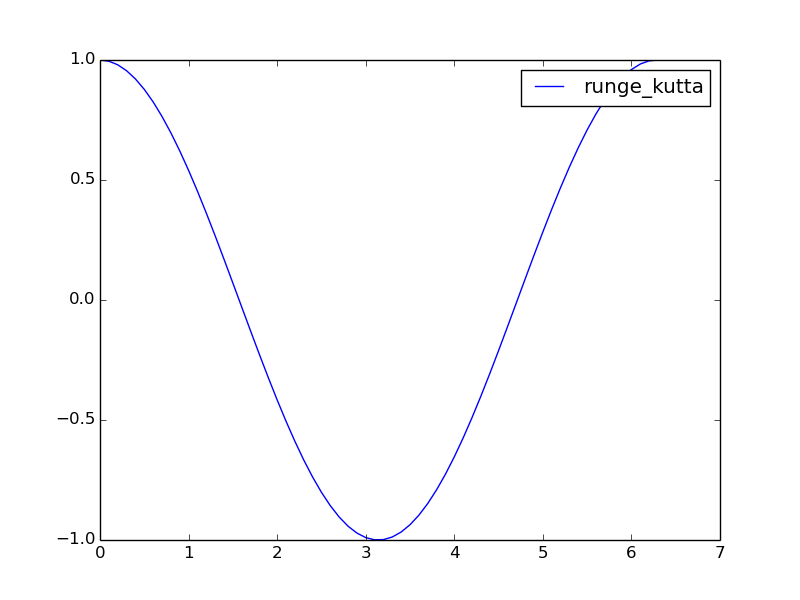
\includegraphics[scale=.5]{fig1_1.png}\hfill
	  	\item For leap frog: \\
	  		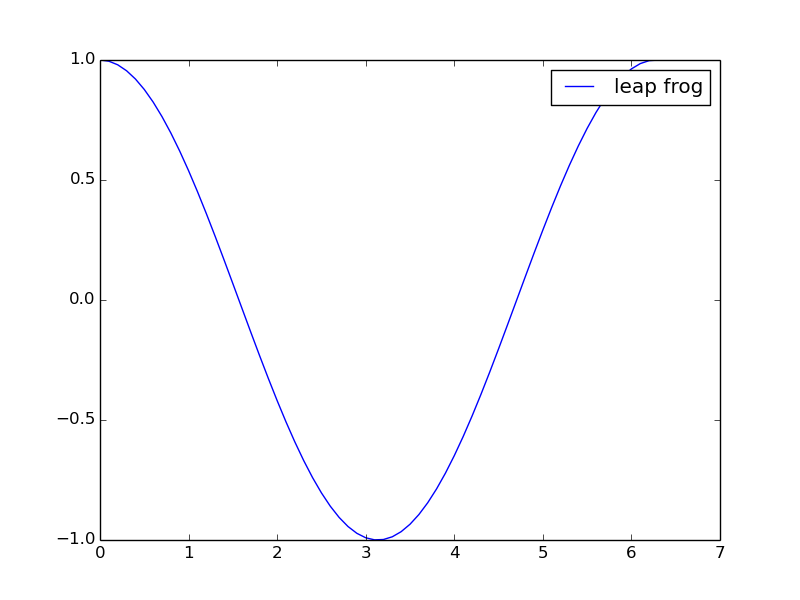
\includegraphics[scale=.5]{fig1_2.png}\hfill

	  	\item The following is a long term plot: \\
	  		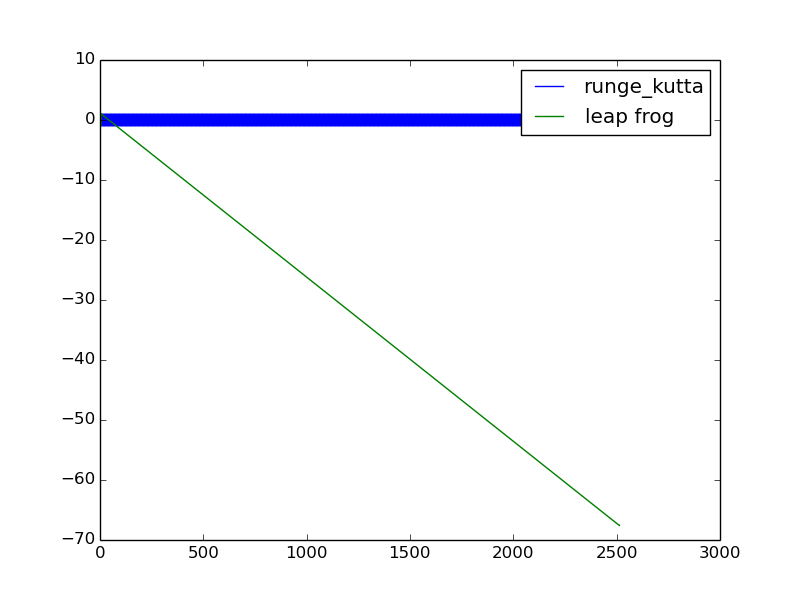
\includegraphics[scale=.5]{fig1_5.png}
	\end{enumerate} 
	For the empirical order of convergence, using the method stated in the previous homework, for Runge-Kutta, the value is about 4.00658215085 and for leap frog, the value is about 2.00169514825.

	\item Refer to script for implementation. The plots for both methods are shown below:\\
	\begin{enumerate}[(i)]
	  	\item For Runge-Kutta: \\
	  		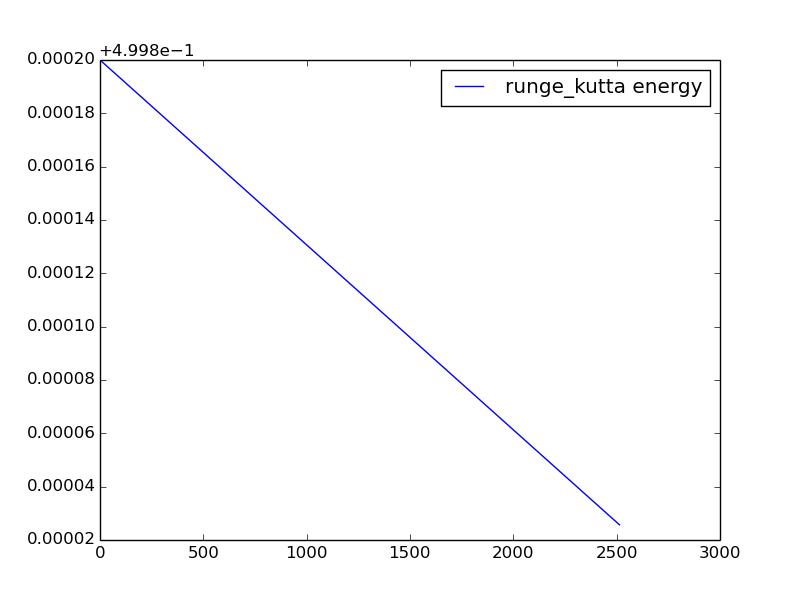
\includegraphics[scale=.5]{fig1_3.png}\hfill
	  	\item For leap frog: \\
	  		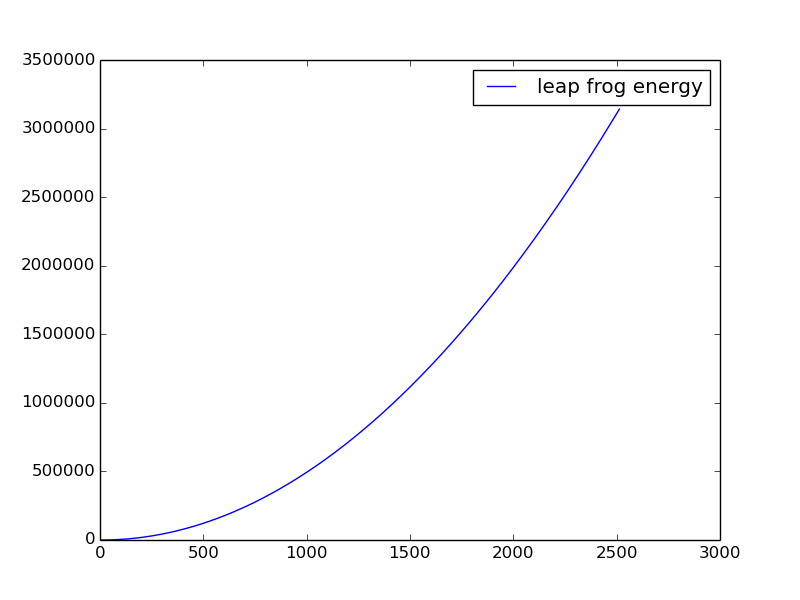
\includegraphics[scale=.5]{fig1_4.png}\hfill
	\end{enumerate} 
	As the plots suggest, we see that the Runge-Kutta method dissipates energy over time whereas the leap frog method amplifies it! The dissipative nature of Runge-Kutta can be problematic for the example given because the model would predict the satellite losing energy overtime which would mean that eventually the earth's gravity would be able to pull it back down. This is an issue because if the dissipative nature of the approximation method is not known beforehand, the satellite may be designed to travel at a faster speed which may cause it escape earth's orbit completely!
\end{enumerate}
\newpage

\begin{center}
	\textbf{Problem 2}
\end{center}

\begin{enumerate}[(a)]
	\item Rewriting the problem as a first-order system of ODEs with separate boundary conditions by writing $x_1 = u$ and $x_2 = x_1'$, we see that the given second-order ODE is the same as the following system of first-order ODES
	\begin{align*}
		x_1' &= x_2 \\
		x_2' &= x_1
	\end{align*}
	with boundary conditions $x_1(0) = \alpha$ and $x_1(b) = \beta$. 

	\item To see that given matrix is indeed the fundamental solution matrix, we must verify that the columns of $\mathbf{Y}$ are solutions to the previous system of ODEs given above and are linearly independent. To verify that they are solutions, observe that if we let $x_1(t) = \cosh(t)$ and $x_2(t) = \sinh(t)$, then indeed we have that 
	\[
		x_1'(t) = \sinh(t) = x_2(t)
	\]
	and 
	\[
		x_2'(t) = \cosh(t) = x_1(t).
	\]
	Similarly, if we let $x_1(t) = \sinh(t)$ and $x_2(t) = \cosh(t)$, then indeed we have that 
	\[
		x_1'(t) = \cosh(t) = x_2(t)
	\]
	and 
	\[
		x_2'(t) = \sinh(t) = x_1(t).
	\]
	For non-singularity, observe that the determinant of $\mathbf{Y}$ is $\cosh^2(t) - \sinh^2(t)$. This quantity evaluates to 1 so the determinant is non-zero so $\mathbf{Y}$ is non-singular. Thus it follows that $\mathbf{Y}$ is the fundamental solution matrix to first-order system given above.

	\item The solutions to this ODE are stable since any solution can be written as a linear combination of the columns given in $\mathbf{Y}$ and those solutions are stable.

	\item To determine the matrix $\mathbf{Q}$, we first need to find out $\mathbf{B_0}$ and $\mathbf{B_b}$. To do this, observe that if $\mathbf{y} = [y_1, y_2]^T$ was a solution to the given boundary value problem, then we would need 
	\[
		\mathbf{B_0 y(0) + B_b y(b) = [\alpha, \beta]}^T.
	\]
	But since $y_1(0) = \alpha$ and $y_1(b) = \beta$, this means that 
	\[
		\mathbf{B_0} =
		\left[
		\begin{tabular}{cc}
		1 & 0\\
		0 & 0
		\end{tabular}
		\right]
	\]
	and
	\[
		\mathbf{B_b} =
		\left[
		\begin{tabular}{cc}
		0 & 0\\
		1 & 0
		\end{tabular}
		\right].
	\]
	Since $\cosh(0) = 1$ and $\sinh(0) = 0$, it follows that
	\[
		\mathbf{Q} = 
		\left[
		\begin{tabular}{cc}
		1 & 0 \\
		$\cosh(b)$ & $\sinh(b)$
		\end{tabular}
		\right].
	\]

	\item To determine the rescaled matrix $\mathbf{\Phi}(t)$, observe first that
	\[
		\mathbf{Q}^{-1} = 
		\left[
		\begin{tabular}{cc}
		1 & 0 \\
		$-\frac{\cosh(b)}{\sinh(b)}$ & $\frac{1}{\sinh(b)}$
		\end{tabular}
		\right].
	\]
	Thus the rescaled matrix is given by
	\[
		\mathbf{\Phi}(t) = 
		\left[
		\begin{tabular}{cc}
		$\cosh(t) - \frac{\sinh(t)\cosh(b)}{\sinh(b)}$ & $\frac{\sinh(t)}{\sinh(b)}$ \\
		$\sinh(t) - \frac{\cosh(t)\cosh(b)}{\sinh(b)}$ & $\frac{\cosh(t)}{\cosh(b)}$
		\end{tabular}
		\right]
	\]

	\item By what was calculated above, we see that as $b$ increases, both the condition number of $\mathbf{Q}$ and the norm of $\mathbf{\Phi}$ increase. This is because $\mathbf{Q}^{-1}$ become increasingly more singular. The solutions, however, will still remain stable as $b$ increases. This is because stability depends only on the stability of the solutions given in the fundamental solutions matrix.
\end{enumerate}
\newpage

\begin{center}
	\textbf{Problem 3}
\end{center}

\begin{enumerate}[(a)]
	\item Refer to script for implementation. 
	
	\item Refer to script for implementation. Consider the plots below: \\
	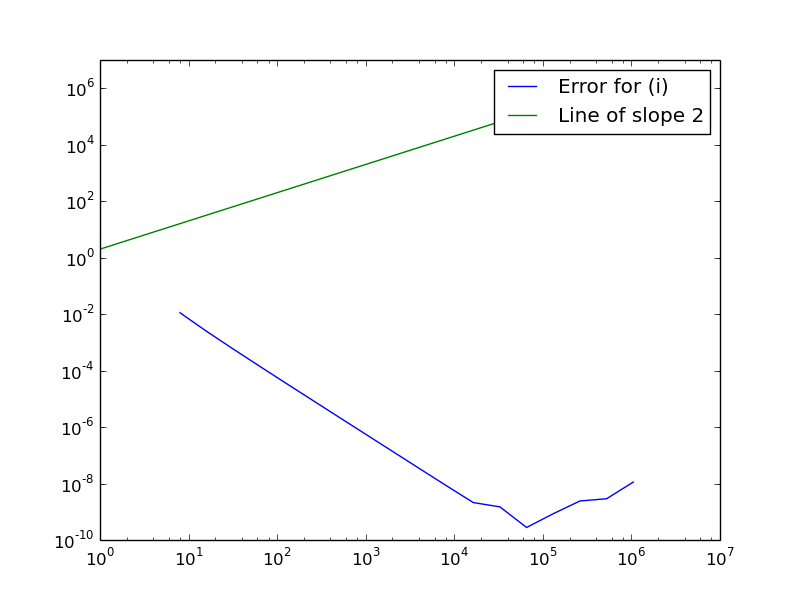
\includegraphics[scale=.5]{fig3_1.png} \hfill \\
	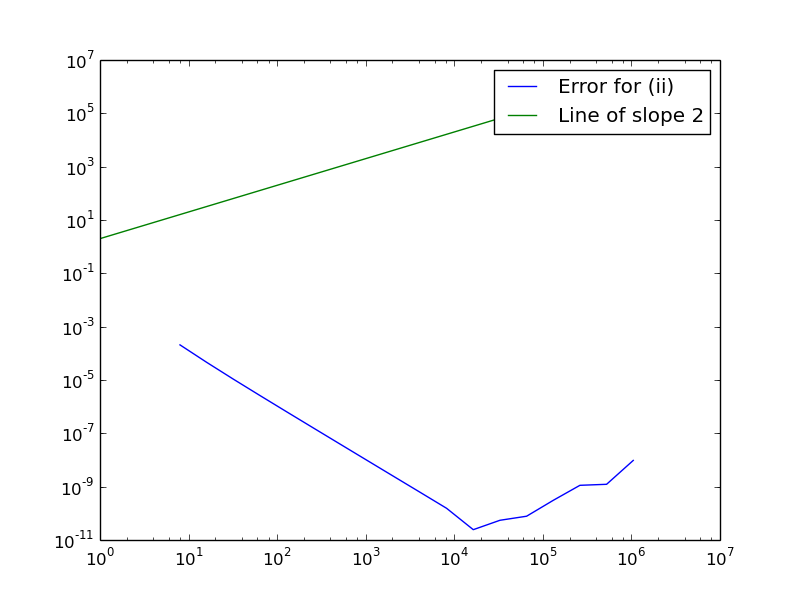
\includegraphics[scale=.5]{fig3_2.png} \hfill \\
	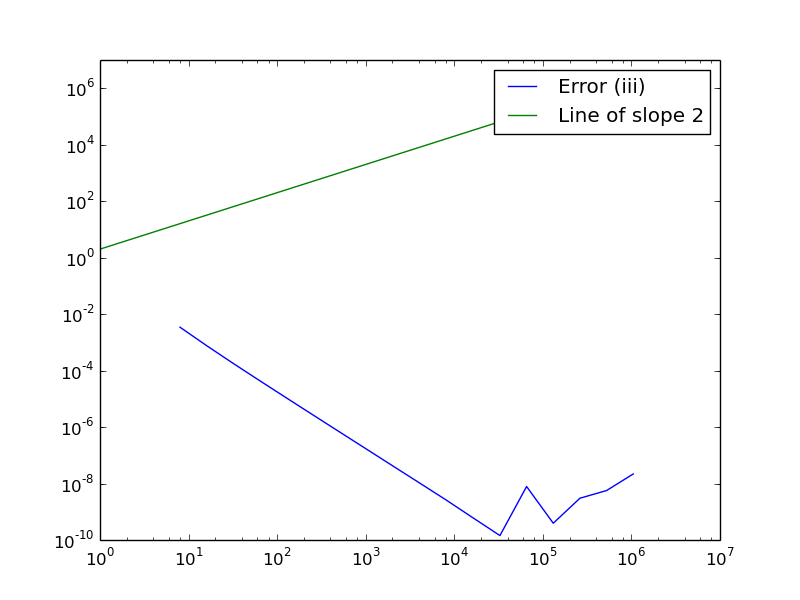
\includegraphics[scale=.5]{fig3_3.png} \hfill \\
	Observe that for each plot, the error does NOT decrease monotonically. After the error reaches around $10^{-10}$, it begins to climb. This is due to the interplay between truncation and rounding error. For large $n$, the step size used is very small so the error is dominated by rounding error whereas for small $n$, the step size is rather large so the error is dominated by truncation error.

	\item Refer to script for implementation. Consider the plot of the condition numbers below: \\
	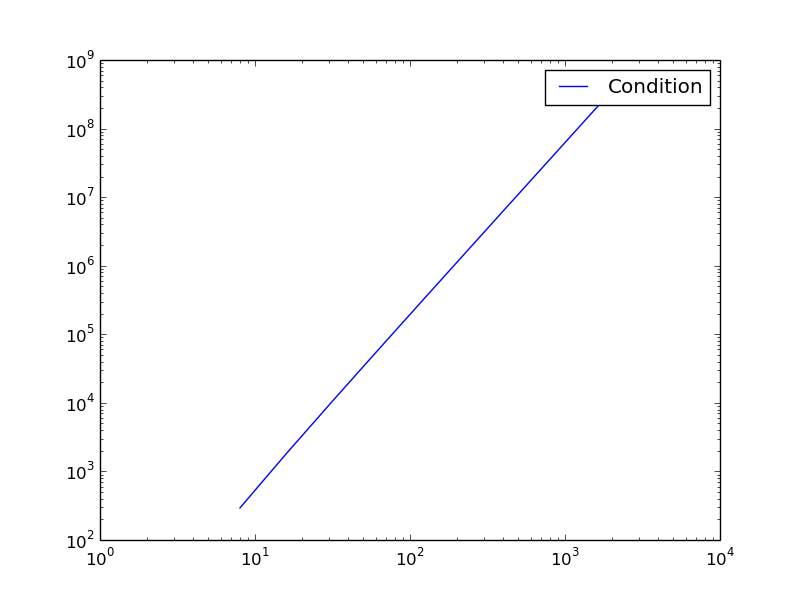
\includegraphics[scale=.5]{fig3_4.png}.\hfill \\
	Observe that the condition number becomes increasingly worse the larger we make $n$.
\end{enumerate}
\newpage
\begin{center}
	\textbf{Problem 4}
\end{center}

\begin{enumerate}[(a)]
	\item Observe that we may write the SOR method in the form:
	\[
		x^{k+1} = (D + \omega L)^{-1}[(1 - \omega)D - \omega U]x^k + \omega(D + \omega L)^{-1}b
	\]
	where $A = D + L + U$ and $D$ is diagonal, $L$ is lower triangular with zeros on the diagonal, and $U$ is upper triangular with zeros on the diagonal.
	We know that an iterative method such as the one above converges only if the coefficient matrix of $x^k$ has spectral radius less than 1. Thus it suffices to study the spectral radius of 
	\[
		(D + \omega L)^{-1}[(1 - \omega)D - \omega U].
	\]
	Observe now that
	\begin{align*}
		\big|\det((D + \omega L)^{-1}[(1 - \omega)D - \omega U])\big|
		&= \big|\det(D + \omega L)^{-1}\det((1 - \omega)D - \omega U)\big| \\
		&= \bigg|\frac{\det(D - \omega(D + U))}{\det(D + \omega L)}\bigg|
		\intertext{Since $L$ is lower triangular with zeros on the diagonal, $\det(D + \omega L)$ is just the product of the diagonal entries of $D$. Denote this product by $d$. Furthermore, since $U$ is upper triangular with zeros on the diagonal, $\det(D - \omega(D + U)) = d(1- \omega)^n$. Thus we see the above is}
		&= \big|1 - \omega\big|^n.
	\end{align*}
	Since the determinant of a matrix is also the product of all its eigenvalues, this means that of the $n$ (not necessarily distinct) eigenvalues $\lambda_j, 1\leq j\leq n$ of $(D + \omega L)^{-1}[(1 - \omega)D - \omega U])$ there must be at least one $\lambda_i$ such that
	\[
		|\lambda_i| \geq |1 - \omega|.
	\]
	This means that the spectral radius of the above matrix is bounded below by $|1 - \omega|$ so the SOR method converges only if 
	\[
		|1 - \omega| < 1
	\]
	which means that the following bound must hold for $\omega$:
	\[
		0 < \omega < 2.
	\]

	\item We show the subspace spanned by the first $m$ search directions in the conjugate gradient method is the same as the Krylov subspace $K_{m}$ generated by the sequence $\mathbf{r_0, Ar_0,\cdots, A^{m-1}r_0}$ by induction on $m$. For the base case, observe that algorithm gives $s_0 = r_0$ so trivially $s_0 \in K_1$. Thus suppose the clam holds for indices greater than $1$ up to $m-1$. We shall show that $s_m \in K_{m+1}$. Observe that by the algorithm, 
	\[
		s_m = r_m + \beta_m s_{m-1}.
	\]
	By the induction hypothesis, $s_{m-1} \in K_{m+1}$ so we need only show that $r_m \in K_{m+1}$. Again by the algorithm, we see that
	\begin{align*}
		r_m 
		&= r_{m-1}  - \alpha_{m-1} \mathbf{A}s_{m-1} \\
		&= r_{m-2} - \alpha_{m-2}\mathbf{A}s_{m-2} - \alpha_{m-1} \mathbf{A}s_{m-1} \\
		&= r_0 - \alpha_{0} \mathbf{A}s_{0} - \cdots - \alpha_{m-1} \mathbf{A}s_{m-1}.
	\end{align*}
	Again by the induction hypothesis, each of the above summands is in $K_{m+1}$ so indeed $r_m \in K_{m+1}$, completing the induction.
	Thus we have shown that the space spanned by the first $m$ search direction is contained the given Krylov subspace. To show that the spaces are indeed the same, we note the fact that each of the $m$ directions are linearly independent to all the other directions. Thus both spaces have the same dimension which then must imply that they are indeed the same space.
\end{enumerate}
\newpage
\begin{center}
	\textbf{Problem 5}
\end{center}

\begin{enumerate}[(a)]
	\item To investigate the stability of all combinations of methods presented, we need only understand the eigenvalues of the finite difference matrix $\mathbf{A}$. 
	\begin{enumerate}[(i)]
		\item Observe that for the centered difference, we get the following eigenvalues plotted on the complex plane: \\
		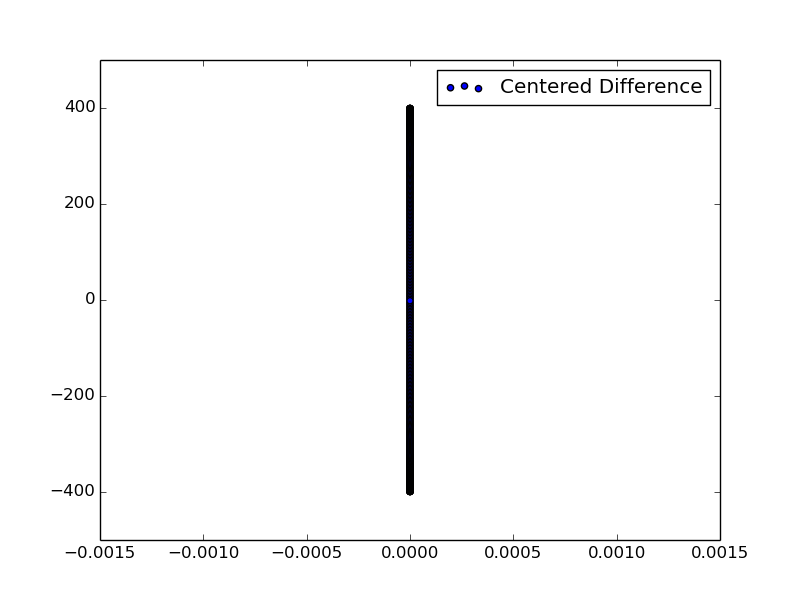
\includegraphics[scale=.5]{fig5_1.png}\hfill \\
		\item Observe that for the upwind method, we get the following eigenvalues plotted on the complex plane: \\
		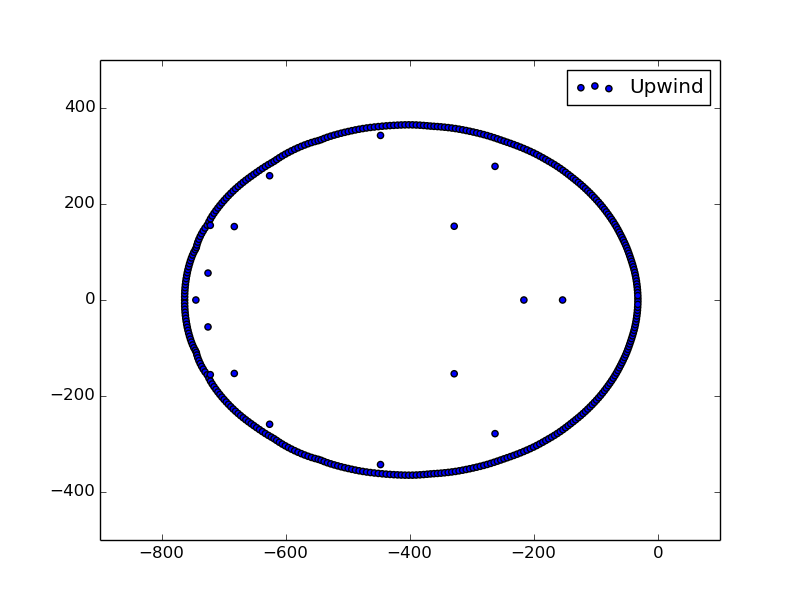
\includegraphics[scale=.5]{fig5_2.png}\hfill \\
	\end{enumerate}
	Combinations of these discretization methods will be stable if the eigenvalues of \textbf{A} fall into the stability regions of the time discretization methods. Using the plots given on the website, we need only scale \textbf{A} until the eigenvalues fall into the correct regions. This scaling factor will determine the correct CFL constant and in turn the right time-step to use. First, we immediately observe that the centered difference method combined with forward-euler cannot be stable since for no scaling factor will all the eigenvalues fall into forward-euler's stability region. For Runge-Kutta, we need the largest and smallest imaginary parts of the eigenvalues of the centered difference method matrix to be around $\pm 2.5$ respectively. As the plot below shows, a CFL constant of .005 gives this to us: \\
	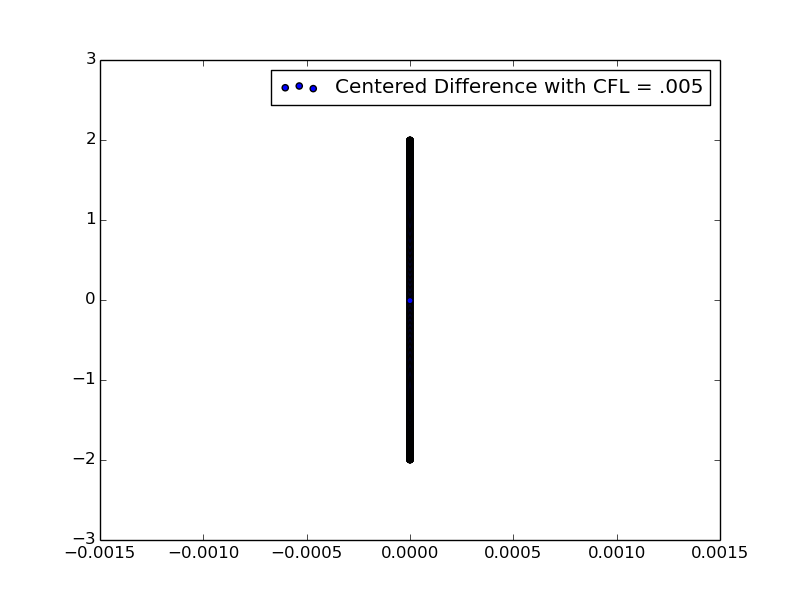
\includegraphics[scale=.5]{fig5_3.png}\hfill\\
	Thus the centered-difference method should be stable with Runge-Kutta with a time step of approximately $\Delta t \approx 1.25\times 10^{-5}$. \\
	Using similar analysis as above, we see that the plot below indicates that for Runge-Kutta, a CFL constant of .003 for the upwind method should be good enough: \\
	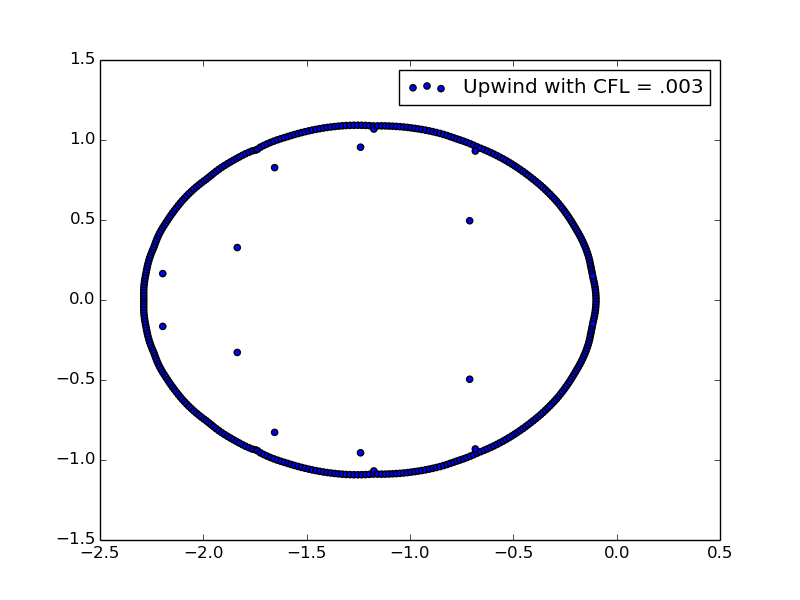
\includegraphics[scale=.5]{fig5_4.png}\hfill\\
	This gives a time-step for stability for upwind with Runge-Kutta of $\Delta t \approx 7.5\times 10^{-6}.$ \\
	Finally, for the upwind method to be stable with forward-euler, we need a CFL constant off approximately .001, as the below plot indicates: \\
	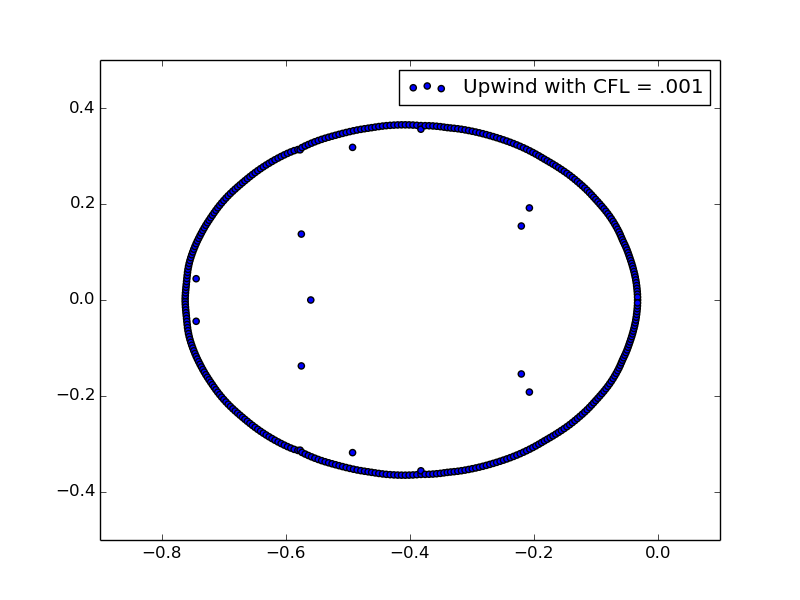
\includegraphics[scale=.5]{fig5_5.png}\hfill \\
	This yields a time step of $\Delta t \approx 2.5\times 10^{-6}.$ 

	\item I was unable to plot the 3d wireframes. I'll consult the solutions when they're out.
\end{enumerate}
	
\end{document}